\documentclass[t, aspectratio=169]{beamer}
\usepackage{amsmath,amsfonts,amsthm,amstext,amssymb, xcolor, tikz, pgf, mathrsfs, polynom, pifont, tabto}

% ----------------------------------------------------------
% Theme Setup

% Use Metropolis Theme
\usetheme[numbering=fraction]{metropolis}
\setbeamertemplate{blocks}[rounded][shadow=false]
\makeatletter
\setlength{\metropolis@titleseparator@linewidth}{1pt}
\makeatother

% Define Colors
\definecolor{chargerblue}{HTML}{002764}
\definecolor{chargerred}{HTML}{e02034}
\definecolor{bggray}{HTML}{d0d3d4}

% Set Colors
\setbeamercolor{title}{fg=chargerblue}
\setbeamercolor{background canvas}{bg=white}
\setbeamercolor{title separator}{fg=chargerred}
\setbeamercolor{structure}{fg=chargerblue}
\setbeamercolor{frametitle}{fg=white, bg=chargerblue}
\setbeamercolor*{normal text}{fg=chargerblue}
\setbeamercolor*{block body}{bg=bggray}
\setbeamercolor*{block title}{bg=chargerblue, fg=white}
% ----------------------------------------------------------

% ----------------------------------------------------------
% Custom Definitions, Commands, Environments, etc.

% Sets of numbers
\def\R{\mathbb{R}} % The reals
\def\N{\mathbb{N}} % The naturals
\def\Z{\mathbb{Z}} % The integers
\def\Q{\mathbb{Q}} % The rationals

% Blank space
\newcommand{\blank}[1]{\underline{\hspace{#1}}} % Blank space

% Change font colors
\newcommand{\cyan}[1]{{\color{cyan}{#1}}} % Changes font to cyan
\newcommand{\red}[1]{{\color{red}{#1}}} % Changes font to red
\newcommand{\magenta}[1]{{\color{magenta}{#1}}} % Changes font to magenta
\newcommand{\orange}[1]{{\color{orange}{#1}}} % Changes font to orange
\newcommand{\yellow}[1]{{\color{yellow}{#1}}} % Changes font to yellow
\newcommand{\violet}[1]{{\color{violet}{#1}}} % Changes font to violet
\newcommand{\green}[1]{{\color{green}{#1}}} % Changes font to green
\newcommand{\blue}[1]{{\color{blue}{#1}}} % Changes font to blue
\newcommand{\white}[1]{{\color{white}{#1}}} % Changes font to white

% Fitted inclusion symbols
\newcommand{\fp}[1]{\left({#1}\right)} % Fitted parentheses around content
\newcommand{\fb}[1]{\left[{#1}\right]} % Fitted brackets
\newcommand{\lhoi}[1]{\left({#1}\right]} % Left half-open interval
\newcommand{\rhoi}[1]{\left[{#1}\right)} % Right half-open interval
\newcommand{\set}[1]{\left\{{#1}\right\}} % Fitted braces (useful for sets)
\newcommand{\av}[1]{\left|{#1}\right|} % Fitted absolute value bars

% Augmented Matrix Environment
\newenvironment{amatrix}[1]{%
	\left[\begin{array}{@{}*{#1}{c}|c@{}}
	}{%
	\end{array}\right]
}

% Miscellaneous
\def\then{\Rightarrow}
\def\to{\rightarrow}
\def\d{^{\circ}}
\newcommand{\?}{\stackrel{?}{=}}
\newcommand{\cmark}{\text{ \ding{51}}}
\newcommand{\xmark}{\text{ \ding{55}}}

% Coordinate Plane (Four-Quadrant)
\def\coordplane {
	\begin{tikzpicture}        \draw[step=0.25cm,black,very thin,opacity=0.25] (-2.5cm, -2.5cm) grid (2.5cm, 2.5cm);
		\draw[<->,thick,black] (-2.5cm, 0) -- (2.5cm, 0) node[anchor=north west,pos=0.94,font=\scriptsize]{$x$};
		\draw[<->,thick,black] (0,-2.5cm) -- (0, 2.5cm) node[anchor=south east,font=\scriptsize,pos=0.94]{$y$};
	\end{tikzpicture}
}

% Coordinate Plane (One-Quadrant)
\def\onequad {
	\begin{tikzpicture}
		\draw[step=0.25cm, black, very thin, opacity=0.25] (0,0) grid (7.5cm,5cm);
		\draw[->, thick, black] (0,0) -- (7.5cm, 0) node[anchor=north west,font=\scriptsize,pos=0.94]{$x$};
		\draw[->, black, thick] (0,0) -- (0,5cm) node[anchor=south east,font=\scriptsize,pos=0.94]{$y$};
	\end{tikzpicture}
}
% ----------------------------------------------------------

% ----------------------------------------------------------
% Presentation Information
\title[7-1]{Confidence Intervals for the Mean when $\sigma$ is Known}
\subtitle{Section 7-1}
\author{Jacob Ayers}
\institute{Lesson \#20}
\date{MAT 110}
% ----------------------------------------------------------

\begin{document}
	
	% Slide 1 (Title Slide)
	\begin{frame}
		\titlepage
	\end{frame}
	
	% Slide 2 (Objectives)
	\begin{frame}{Objectives}
		\begin{itemize}
			\item Construct confidence intervals for the mean when $\sigma$ is known
		\end{itemize}
	\end{frame}

	\begin{frame}{Estimation}
		Today's Goal: Estimate the population mean, when we know the mean of a sample and also the population standard deviation $\sigma$. \pause
		
		A \textit{point estimate} is a specific numerical value estimate of a parameter. \pause \\
		The best point estimate of the population mean $\mu$ is the sample mean $\overline{X}$.
		
		Example: Average age of students in this class is approximately 17.8. I use this to estimate that the mean age of all freshman students at Carl Sandburg College is 17.8.
		
		We call the sample mean an \textit{estimator} in this instance.
	\end{frame}

	\begin{frame}{Estimation}
		An \textit{estimator} is a sample statistic that is used to estimate a population measure. \pause
		
		Good estimators meet the following criteria: \pause
		
		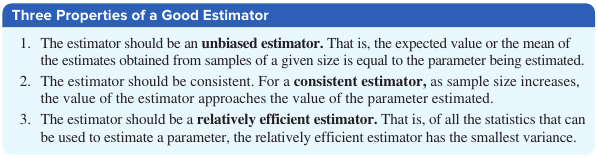
\includegraphics[width=\textwidth]{good-estimator.png}
	\end{frame}

	\begin{frame}{Estimation}
		We have previously discussed that the sample mean will usually differ from the population mean due to sampling error. \pause
		
		Question: How good is a point estimate? \pause \\
		Answer: There's no way to know for sure. \pause
		
		This is a problem, as it calls into question the accuracy of point estimates. \pause
		
		Solution: Cast a wider net by using an interval estimate. \pause
		
		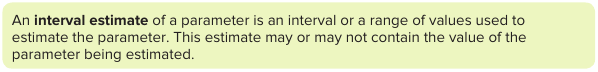
\includegraphics[width=\textwidth]{ie-def.png} \pause
		
		Example: Instead of estimating average age to be 17.8, estimate it to be $17.3 < \mu < 18.3$ (or $17.8 \pm 0.5$)
	\end{frame}

	\begin{frame}{Confidence Intervals}
		Before we make an interval estimate, we start by assigning a degree of confidence (usually a percentage) that the population parameter will actually be in the interval. \pause
		
		The most commonly used confidence levels are 90\%, 95\%, and 99\%. \pause Why not always 99\%? \pause
		
		Answer: There's a tradeoff between degree of confidence and width of the interval estimate. \pause
		
		If you want to be more confident that the parameter will be in the interval, then you need to make the interval wider. \pause 
	\end{frame}

	\begin{frame}{Confidence Intervals}
		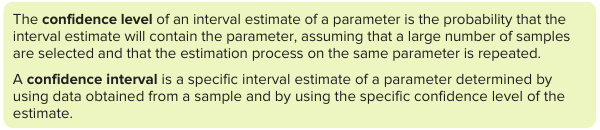
\includegraphics[width=\textwidth]{conf-defs.png} \pause
		
		Graphing calculators will find confidence intervals (you can determine how online, if interested), but I'll be showing it ``by hand."
	\end{frame}

	\begin{frame}{Confidence Intervals}
		The Central Limit Theorem states that when $n$ is large, approximately 95\% of sample means taken from a population will fall within 1.96 standard errors of the population mean (i.e. $\mu \pm 1.96(\sigma/\sqrt{n})$). \pause
		
		Likewise, there is a 95\% probability that the interval specified by $\overline{X} \pm 1.96(\sigma/\sqrt{n})$ will contain $\mu$. \pause
		
		So a 95\% confidence interval will be of the form $$\overline{X} - 1.96(\sigma/\sqrt{n}) < \mu < \overline{X} + 1.96(\sigma/\sqrt{n}).$$ \pause
		
		If the confidence level isn't 95\%, we will use the constant associated with that confidence level in the $z$ table instead of 1.96.
	\end{frame}

	\begin{frame}{Confidence Intervals}
		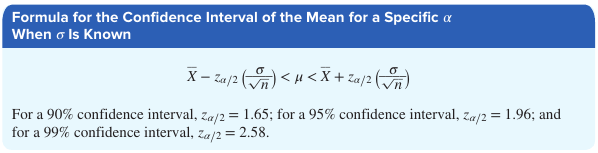
\includegraphics[width=\textwidth]{ci-formula.png} \pause
		
		We call $z_{\alpha / 2}\fp{\dfrac{\sigma}{\sqrt{n}}}$ the \textit{margin of error} of the estimate. \pause
		
		When we find these confidence intervals, we are operating under two assumptions: \begin{enumerate}[1)]
			\item The sample is a random sample.
			\item Either the sample size is 30 or more, or normally distributed if not
		\end{enumerate}
	\end{frame}

	\begin{frame}{Confidence Intervals}
		Let's run through a explanation using a visual before we start finding these confidence intervals.
		
		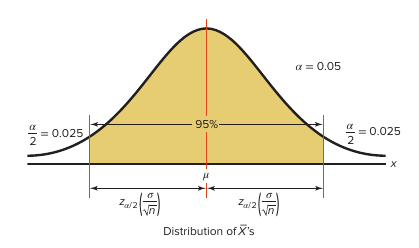
\includegraphics[width=4in]{ci-visual.png}
	\end{frame}

	\begin{frame}{Constructing Confidence Intervals}
		To construct a confidence interval when $\sigma$ is known: \begin{enumerate}[1)]
			\item Make sure the assumptions are met. \pause
			\item Evaluate $\dfrac{\sigma}{\sqrt{n}}$; store the result in your calculator. \pause
			\item Look up $1 - \alpha / 2$ in the standard normal table; this is $z_{\alpha/2}$ \pause
			\item Use the formula $$\overline{X} - z_{\alpha/2}\fp{\dfrac{\sigma}{\sqrt{n}}} < \mu < \overline{X} - z_{\alpha/2}\fp{\dfrac{\sigma}{\sqrt{n}}}$$ to write the confidence interval
		\end{enumerate}
	\end{frame}

	\begin{frame}{Constructing Confidence Intervals}
		A researcher wishes to estimate the number of days it takes an automobile dealer to sell a Chevrolet Aveo. A random sample of 50 cars had a mean time on the dealer's lot of 54 days. Assume the population standard deviation to be 6.0 days. Find a 90\% confidence interval of the population mean. \pause
		
		1) The assumptions hold. This is a random sample, and $n = 50 \geq 30$. \pause \\
		2) Using a calculator, $\dfrac{\sigma}{\sqrt{n}} = \dfrac{6.0}{\sqrt{50}} \approx 0.8485281374$; store this value \pause \\
		3) Since this is a 90\% confidence interval, $\alpha = 1 - 0.9000 = 0.1000$. Then $1 - \alpha / 2 = 1 - 0.0500 = 0.9500$. \pause $z_{\alpha/2}$: 1.65 \pause
		
		4) Lower Limit for CI: $54 - 1.65(0.8485) \approx 52.6$ \pause \\
		Upper Limit for CI: $54 + 1.65(0.8485) \approx 55.4$ \pause
		
		So the 90\% confidence interval is: $52.6 < \mu < 55.4$
	\end{frame}

	\begin{frame}{Constructing Confidence Intervals}
		The following data represent a random sample of the assets (in millions of dollars) of 30 credit unions in southwestern Pennsylvania. Assume the population standard deviation is 14.405. Find the 99\% confidence interval of the mean.
		
		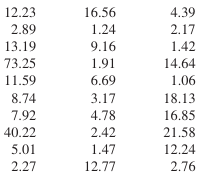
\includegraphics[width=1.5in]{pa-data.png} \pause
		
		1) The assumptions hold. This is a random sample, and $n \geq 30$. \pause
		
		Before continuing, we need to find $\overline{X}$. Using a calculator, $\overline{X} \approx 11.091$.
	\end{frame}

	\begin{frame}{Constructing Confidence Intervals}
		Important Information: $n = 30$, $\sigma = 14.405$, $\overline{X} = 11.091$
		
		2) Using a calculator, $\dfrac{\sigma}{\sqrt{n}} = \dfrac{14.405}{\sqrt{30}} \approx 2.629981147$; store this value. \pause
		
		3) Look up $1 - 0.0500/2 = 0.9750$\pause; $z_{\alpha/2} = 1.96$ \pause
		
		4) Lower Limit for CI: $11.091 - 1.96(2.6300) \approx 5.936$ \pause \\
		Upper Limit for CI: $11.091 + 1.96(2.6300) \approx 16.246$ \pause
		
		So the 95\% confidence interval is: $5.936 < \mu < 16.246$
	\end{frame}

	\begin{frame}{Constructing Confidence Intervals}
		For a random sample of 60 overweight men, the mean of the number of pounds they were overweight was 30. The standard deviation of the population is 4.2 pounds. Find the 93\% confidence interval of the mean of the excess pounds they weighed. \pause
		
		1) The assumptions hold. This is a random sample, and $60 \geq 30$. \pause \\
		2) Using a calculator, $\dfrac{\sigma}{\sqrt{n}} = \dfrac{4.2}{\sqrt{60}} \approx 0.5422176685$; store this value \pause \\
		3) Look up $1 - 0.07/2 = 0.9650$\pause; $z_{\alpha/2} = 1.81$ \pause
		
		4) Lower Limit for CI: $30 - 1.81(0.5422) \approx 29.02$ \pause \\
		Upper Limit for CI: $30 + 1.81(0.5422) \approx 30.98$ \pause
		
		So the 93\% confidence interval is: $29.02 < \mu < 30.98$
	\end{frame}

	\begin{frame}{Determining Sample Size}
		A commonly asked question in statistics: How big a sample do I need to collect in order to make an accurate estimate? \pause
		
		The answer depends on three things: \begin{enumerate}[1)]
			\item How big of a margin of error are you willing to accept? \pause
			\item What is the population standard deviation? \pause
			\item How confident do you want to be? \pause
		\end{enumerate}
	
		We can use the margin of error formula $E = z_{\alpha / 2}\fp{\dfrac{\sigma}{\sqrt{n}}}$ to derive a formula for the sample size needed for a given confidence level and margin of error.
	\end{frame}

	\begin{frame}{Determining Sample Size}
		\begin{flalign*}
			\onslide<1->{E &= z_{\alpha / 2}\fp{\dfrac{\sigma}{\sqrt{n}}} &  \text{(margin of error formula)}\\}
			\onslide<2->{E(\sqrt{n}) &= z_{\alpha / 2}\cdot \sigma & \text{(multiply by $\sqrt{n}$)} & \\}
			\onslide<3->{\sqrt{n} &= \dfrac{z_{\alpha / 2} \cdot \sigma}{E} & \text{(divide by $E$)} & \\}
			\onslide<4->{n &= \fp{\dfrac{z_{\alpha / 2 \cdot \sigma}}{E}}^2 & \text{(square each side)}}
		\end{flalign*}
	
		\onslide<5->{Rounding Rule: Always round up to nearest whole number (e.g. $65.03 \uparrow 66$)}
	\end{frame}
	
	\begin{frame}{Determining Sample Size}
		A sociologist wishes to estimate the average number of automobile thefts in a large city per day within 2 automobiles. He wishes to be 99\% confident, and from a previous study the standard deviation was found to be 4.2. How many days should he select to survey?
		
		\onslide<2->{We have $\sigma = 4.2$ and $E = 2$.}
		\onslide<3->{Looking up $1 - 0.01/2 = 0.9950$, we find $z_{\alpha/2} = 2.58$}
		\begin{flalign*}
			\onslide<4->{n &= \fp{\dfrac{z_{\alpha / 2} \cdot \sigma}{E}}^2 & \\}
			\onslide<5->{&= \dfrac{2.58 \cdot 4.2}{2}^2} & \\
			\onslide<6->{&= 5.418^2} & \\
			\onslide<7->{&\approx 29.35}
		\end{flalign*}
		\onslide<8->{So he should sample 30 days.}
	\end{frame}

	\begin{frame}{Determining Sample Size}
		A researcher wishes to estimate the average number of minutes per day a person spends on the Internet. How large a sample must she select if she wishes to be 90\% confident that the population mean is within 10 minutes of the sample mean? Assume the population standard deviation is 42 minutes.
		
		\onslide<2->{$\sigma = 42$, $E = 10$; $z_{\alpha/2} = 1.65$}
		\begin{flalign*}
			\onslide<3->{n &= \fp{\dfrac{z_{\alpha/2}\cdot\sigma}{E}}^2 & \\}
			\onslide<4->{&= \fp{\dfrac{1.65(42)}{10}}^2 & \\}
			\onslide<5->{&= 6.93^2} & \\
			\onslide<6->{&\approx 48.02}
		\end{flalign*}
		\onslide<7->{So the sample size should be 49.}
	\end{frame}

	\begin{frame}{Next Steps}
		\begin{itemize}
			\item Complete Assignment \#10
			\item Begin Module \#11 \begin{itemize}
				\item Read 7-2
				\item Watch Video Lesson \#22
			\end{itemize}
		\end{itemize}
	
		\vfill
		
		Thanks for watching!
	\end{frame}
	
\end{document}